\section{Implementácia}
\subsection{Pripínanie trasy k cestnej sieti}

\indent \indent Ukladanie trás spracovaných funkciou map-match, rovnako ako ukladanie pôvodných bodov trás prebieha pomocou skriptu, ktorý je implementovaný v \textit{Python}. Tento skript dostane na vstup slovník, ktorý obsahuje konfiguračné nastavenia skriptu, ako aj parametre pripínania trás k cestnej sieti. Medzi nastavenia skriptu patrí:
\begin{itemize}
  \item unzipdir - cesta k priečinku, ktorý má byť spracovaný map-match algoritmom
  \item container - názov \textit{Valhalla} kontajnera, ktorý poskytuje map-match funkcionalitu.
  \item user - meno používateľa, ktorý nahral súbor alebo požiadal o znovu-spustenie algoritmu
  \item zipname - názov nahraného ZIP súboru
  \item parameters - vnorený slovník, ktorý obsahuje parametre pripínania trás k cestnej sieti.
\end{itemize}

Po načítaní nastavení skriptu prebehne inicializácia pomocných premenných, do ktorých sa bude ukladať priebeh pripnutia trás k cestnej sieti. Inicializuje sa \textit{successful} premenná, ktorá reprezentuje pole, do ktorého sa budú ukladať názvy úspešne spracovaných trás. Taktiež sa inicializuje \textit{failed} premenná, ktorá reprezentuje slovník, do ktorého sa budú ukladať názvy neúspešne spracovaných trás ako kľúče a textový reťazec informujúci o chybe, ktorá nastala ako hodnotu ku kľúču.

Po inicializácií prebehne kontrola \textit{unzipdir} nastavenia. Kontroluje sa, či zadaná cesta odkazuje na priečinok, ktorý obsahuje len priečinky. V prípade, že cesta odkazuje na priečinok, ktorý obsahuje súbor, algoritmus končí a výstupom algoritmu je slovník, ktorý obsahuje chybovú hlášku \textit{``\textbf{názov\textunderscore súboru} is not a directory, check the zip structure.''}, ktorá je neskôr zobrazená používateľovi. Ďalej sa kontrolujú názvy podpriečinkov, ktoré priečinok s cestou \textit{unzipdir} obsahuje. Ak sa v priečinku nachádza priečinok s názvom iným ako \textit{Walk} alebo \textit{Drive}, algoritmus končí a výstupom je slovník, ktorý obsahuje chybovú hlášku ``\textit{\textbf{názov\textunderscore podpriečinku} does not match the specified directory name 'Walk' or 'Drive', check the zip structure.}'' Následne sa prechádzajú jednotlivé súbory (trasy) najprv v \textit{Drive} priečinku, neskôr v \textit{Walk} priečinku. Skript na základe mena súboru identifikuje, o aký typ súboru ide a podľa toho načíta body trasy do premennej. Skript dokáže načítať body z \textit{csv}, \textit{geojson} a \textit{gpx} súboru. V prípade, že je súbor iného typu, do premennej \textit{failed} sa uloží meno trasy ako kľúč a chybová hľáška \textit{``Points couldn't be extracted.''}  ako hodnota.

Po načítaní bodov do premennej vstupuje táto premenná do funkcie map-match. Do tejto funkcie vstupujú aj ďalšie argumenty: \textit{container}, \textit{parameters} a \textit{costing}. Premenná \textit{costing} je určuje typ dopravy a je nastavená na základe priečinka, z ktorého bola trasa načítaná. Ak bola trasa načítaná z priečinka \textit{Walk}, ide o pešiu chôdzu a do premennej sa uloží hodnota \textit{pedestrian}. V opačnom prípade sa do nej uloží hodnota \textit{auto}, reprezentujúca jazdu autom. Premenná \textit{parameters} reprezentuje slovník parametrov pripínania trás k cestnej sieti. Patria sem parametre, ktoré určujú presnosť \acrshort{gps} zariadenia v metroch, ktorým bola trasa meraná, dĺžku polomeru kruhu, v ktorom sa majú hladať kandidáti cestnej siete, ku ktorým sa má bod v trase pripnúť, taktiež v metroch a penalizácia odbáčania na druhú cestu určená celočíselnou hodnotou. Vo funkcii sa naformátujú body spolu s parametrami a druhom dopravy do textového reťazca, ktorý je vložený do požiadavky na \textit{Valhalla} kontajner. Ukážku textového reťazca je možné vidieť vo výpise \ref{lst:request}.
\begin{lstlisting}[
    caption={Dáta požiadavky na \textit{Valhalla} kontajner},
    label={lst:request}
  ]
  {
    "shape": [{"lat": 47.993351,"lon": 18.174553},{"lat": 47.993351,"lon": 18.174553}],
    "shape_match": "map_snap",
    "costing": "auto",
    "costing_options": {"pedestrian": {"ignore_access": true}},
    "format": "osrm",
    "trace_options": {
        "search_radius": 50,
        "turn_penalty_factor": 200,
        "gps_accuracy": 5
    }
}
  \end{lstlisting}
Je možné vidieť jednotlivé parametre pripínania a ostatné nastavenia. Nastavenie \textit{ignore\textunderscore access} pre pešiu chôdzu nastavujeme, aby sme algoritmu oznámili, že má ignorovať typy ciest pri hľadaní kandidátov cestnej siete, ku ktorým má trasu pripnúť. Vďaka tomuto nastaveniu môže algoritmus pripnúť pešiu chôdzu aj na cyklotrasu.

Po odoslaní požiadavky na \textit{Valhalla} kontajner a prijatí odpovede funkcia vráti odpoveď, ktorá je neskôr spracovaná. Z ukážky \ref{lst:response} možno vidieť, že trasa je zložená z rôznych segmentov, označenými atribútom \textit{legs}. V ukážke \ref{lst:response} je zobrazený len jeden segment, aby výpis nebol zbytočne veľký. Je možné vidieť, že geometria nájdenej trasy obsahuje geometriu z prvého segmentu v \textit{legs} atribúte.

\begin{lstlisting}[
    caption={Odpoveď z \textit{Valhalla} kontajnera},
    label={lst:response}
  ]
  {
    {
    "matchings": [
        { "weight_name": "pedestrian", "weight": 10027.532, "duration": 7257.535, "distance": 10239.001,
          "legs": [{
                    "via_waypoints": [], "admins": [ {} ], "weight": 10027.532, "duration": 7257.535,
                    "steps": [ { 
                        "intersections": [ 
                            { "bearings": [ 253 ], "entry": [ true ], "admin_index": 0, "out": 0, "geometry_index": 0, "location": [ 17.063915, 48.158126 ] } 
                            ],
                        "maneuver": {
                            "instruction": "Walk west.",
                            "type": "depart",
                            "bearing_after": 253,
                            "bearing_before": 0,
                            "location": [ 17.063915, 48.158126 ]
                        },
                        "name": "",
                        "duration": 4.941,
                        "distance": 7,
                        "driving_side": "left",
                        "weight": 4.941,
                        "mode": "walking",
                        "geometry": "{yizzAu}np_@b@rD"
                    }],
                    "distance": 10239.001,
                    "summary": "Stare Grunty, Dvorakovo nabrezie"
                }
            ],
            "geometry": 
                "{yizzAu}np_@b@rDxHaD~GsGjHiH|BsBpAdAgFnUs@~CzIoClp@mSni@}Oj\\kJt@UltBun@jLgD|\\gKnKaG~QyKrBaA~
                EoCjK{GfNgKzLcK~AcC~CqFxc@{j@jIoKrB}CjGiJxt@q`AlLKjLbCtSlCbEeCtDiGr@}J~@_b@NcHRyIhByz@|@e`@f@}T
                VcJhL^hJl@tETlIh@d@mSt@DcA|c@GdA_AYq@GhAmd@f@gJh@ag@z@g^pAiQjCaQbAaEhAeDbEkKdBgEhCkEhByBdDoC`Ri
                MnAg@bEk@`@UTq@jBmFvBiGXYjAgAfPuArBn@hSvFdYbIjFtAjh@vN|InCdGh@NiEd@gNeAGD{A@]Bu@HuBhAJGvBEpAw@I
                DqADwAr@}Wf~Hny@jw@fHla@tBBg@@]lLl@F_BkYmBiEu]sHio@{CcWcCcWkAkQgA{WYyNO{N@yMHsM\\sOt@qQr@yL`A}L
                dCgV|C_VzFgc@bs@qsF|m@omGxs@ynHbC_WjAoZVqSEkS_AeZkBkZeD{W_Gq]}BuN_BoNaAeRUgO~AexAJuKnA{jAm@wSgB
                qNiCyNgGiSmAkHQoCYeEqIsmBMkCo@wMh@A|@CnEK?}@egEpHs^gAq@CAeLj@?x@ACuKAgCbJYnC?bA?r@?v@?p@?hA?rC?
                fAhJDbTFzPBrNgC|zA}AjrA_BxrA_|@}Iht@kIrw@", "confidence": 1
        }
    ],
    "tracepoints": [
        {
            "matchings_index": 0, "waypoint_index": 0, "alternatives_count": 0,
            "distance": 43.15, "name": "", "location": [ 17.063915, 48.158126 ]
        }, { ... }
    ],
    "code": "Ok"
    } 
}
  \end{lstlisting}

Z odpovede získame atribút \textit{geometry}, ktorý reprezentuje zakódovanú geometriu cestnej siete, po ktorej sa predpokladá, že používateľ prechádzal. Geometria sa dekóduje na body, ktoré sú uložené do súboru s názvom \textit{map-match.csv}. Pôvodné body sú uložené do súboru s názvom \textit{original.csv}. Tieto dva súbory sú potom uložené do priečinka \textit{routes} pre príslušného používateľa, príslušný nahraný súbor a príslušnú trasu. Viac o štruktúre \textit{routes} priečinka je popísané v kapitole \ref{section:saving-files}.

Nakoniec sa inicializuje premenná \textit{retDict}, ktorá bude reprezentovať slovník. Príklad \textit{retDict} premennej vidno na výpise \ref{lst:retdict}, obsahuje nasledujúce kľúč-hodnota páry:
\begin{itemize}
  \item failed -  počet neúspešne spracovaných trás
  \item successful - počet úspešne spracovaných trás
  \item failed-info - premenná \textit{failed}, ktorá obsahuje názov trasy ako kľúč a textový reťazec s informáciou o chybe, ktorá nastala ako hodnotu
\end{itemize}

Výstupom skriptu je premenná \textit{retDict} konvertovaná na textový reťazec. Informácie zo slovníka sú neskôr zobrazené používateľovi, aby v prípade neúspešného pripnutia trás dostal informáciu o chybe a chybnej trase.




\begin{lstlisting}[
    caption={\textit{retDict} premenná},
    label={lst:retdict}
  ]
  {
    {
        "failed": 3,
        "successful": 519,
        "failed_info": {
            "u16112023_187923-189171_2024-01-13200431": "b'{\"code\":\"NoRoute\",\"message\":\"Impossible route between points\"}'",
            "u16112023_74346-75016_2023-12-09121131": "b'{\"code\":\"NoSegment\",\"message\":\"One of the supplied input coordinates could not snap to street segment.\"}'",
            "u16112023_85191-85958_2023-12-09151521": "b'{\"code\":\"NoSegment\",\"message\":\"One of the supplied input coordinates could not snap to street segment.\"}'"
        }
    }
}
  \end{lstlisting}


\subsection{Webová aplikácia}
\subsubsection{Autentifikácia}
\indent \indent Po otvorení webovej aplikácie je používateľovi zobrazená stránka, na ktorej sa musí autentifikovať. Pre použitie aplikácie je potrebné, aby sa používateľ zaregistroval a neskôr prihlásil. Pri registrácii je nutné zadať používateľské meno, ktoré musí byť unikátne. To znamená, že nemôžu existovať dvaja používatelia s tým istým používateľským menom. Pri pokuse o registráciu používateľského mena, ktoré je už registrované, je používateľovi zobrazená chybová hláška viditeľná na obrázku \ref{fig:username-already-exists}. Pri registrácii je taktiež nutné zadať heslo. Heslo je nutné zopakovať znova, aby sa predišlo prípadným chybám alebo preklepom v ňom. Pri pokuse o registráciu s nezhodnými heslami je používateľovi zobrazená chybová hláška viditeľná na obrázku \ref{fig:passwords_dont_match}.

\begin{figure}[H]
  \centering
  \begin{subfigure}{.45\textwidth}
    \centering
    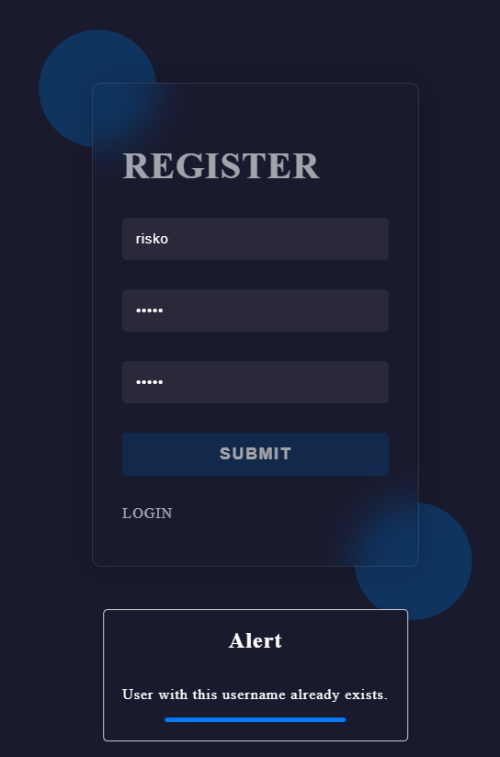
\includegraphics[width=.9\textwidth]{img/auth/username_already_exists.png}
    \caption{Chybová hláška pri pokuse o registráciu existujúceho používateľského mena.}
    \label{fig:username-already-exists}
  \end{subfigure}
  \begin{subfigure}{.45\textwidth}
    \centering
    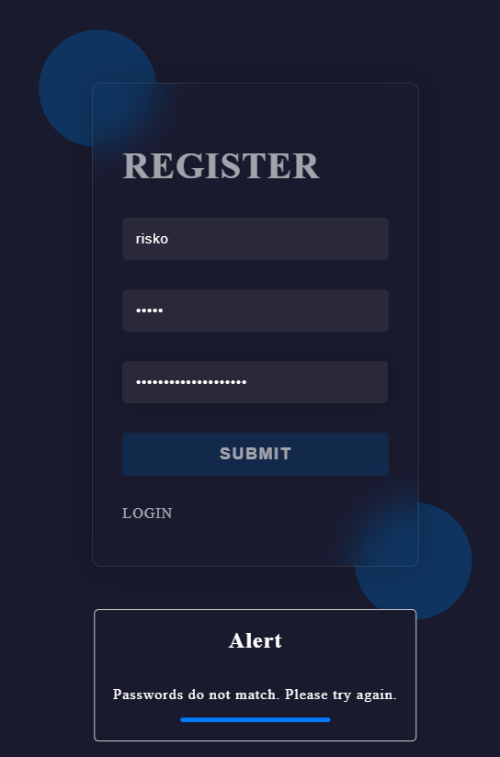
\includegraphics[width=.9\textwidth]{img/auth/passwords_dont_match.png}
    \caption{Chybová hláška pri pokuse o registráciu s nezhodnými heslami.}
    \label{fig:passwords_dont_match}
  \end{subfigure}
  \caption{Možné chybové hlášky pri registrácií pri chybe používateľa.}
\end{figure}

Chyba môže nastať aj na strane aplikácie, napríklad ak je databáza nedostupná alebo nie je zapnutá. Pri vypnutej alebo nedostupnej databáze sa zobrazí chybová hláška zobrazená na obrázku \ref{fig:database_error}. Pri inej možnej chyba sa zobrazí chyba podobne s chybovým kódom.

\begin{figure}[H]
  \centering
  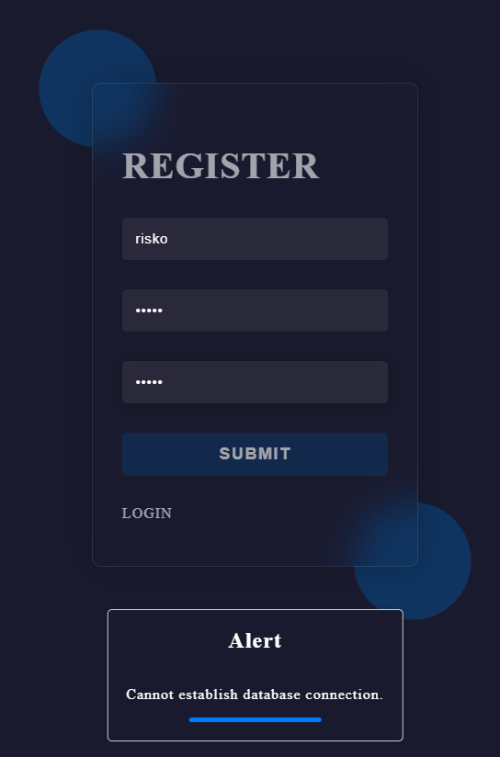
\includegraphics[width=0.5\textwidth]{img/auth/database_error.png}
  \caption{Chybová hláška pri nedostupnej databáze.}
  \label{fig:database_error}
\end{figure}

Po vyplnení údajov a kliknutí na tlačidlo \textit{Submit} sú údaje z polí vložené do požidavky, ktorá je odoslaná na server. Na serveri sa z požiadavky extrahuje meno a heslo. Heslo je \textit{zahashované} pomocou knižnice \textit{Bcrypt}\cite{nodejs-bcrypt}. \textit{Zahashované} heslo je spolu s používateľským menom vložené do databázy. Pri chybe, napríklad duplicitnom zázname používateľského mena, nastane konflikt a databáza vygeneruje chybovú hlášku, ktorá je spracovaná a zobrazená používateľovi. Pri správnom vložení údajov do databázy je používateľ presmerovaný na stránku prihlásenia.

Na stránke prihlásenia používateľ zadá používateľské meno a heslo. Po kliknutí na tlačidlo \textit{Submit} sú údaje vložené do požiadavky, ktorá je odoslaná na server. Tieto údaje sú na serveri extrahované z požiadavky. Na databázu je vytvorený dotaz s používateľským menom. V prípade, že sa používateľské meno nenachádza v databáze, používateľovi je zobrazená chybová hláška \textit{``Invalid username or password''}. V prípade, že sa používateľské meno nachádza v databáze, heslo z požiadavky je \textit{zahashované} pomocou \textit{Bcrypt} funkcie a porovnané so \textit{zahashovaným} heslom z databázy. V prípade, že sa heslá rovnajú, je používateľ presmerovaný na stránku s mapou. V opačnom prípade je používateľovi zobrazená hláška \textit{``Invalid username or password''}.

\subsubsection{Stránka s mapou}

Po autentifikácií je používateľ presmerovaný na stránku s mapou. Stránka je zložená z troch vždy viditeľných častí a šiestich častí viditeľných na základe akcií vykonaných používateľom. Tieto časti stránky sú vytvorené pomocou \textit{div} \acrshort{html} tagov. \textit{Div} tagy slúžia na definovanie rozdelenia stránky alebo sekcií na stránke. Vždy viditeľné časti stránky sú zobrazené na obrázku \ref{fig:map} a sú vyznačené farebnými obdĺžnikmi:
\begin{itemize}
  \item mapa - žltý obdĺžnik
  \item tlačidlá na priblíženie mapy - fialový obdĺžnik
  \item panel akcií - modrý obdĺžnik
\end{itemize}
\begin{figure}[H]
  \centering
  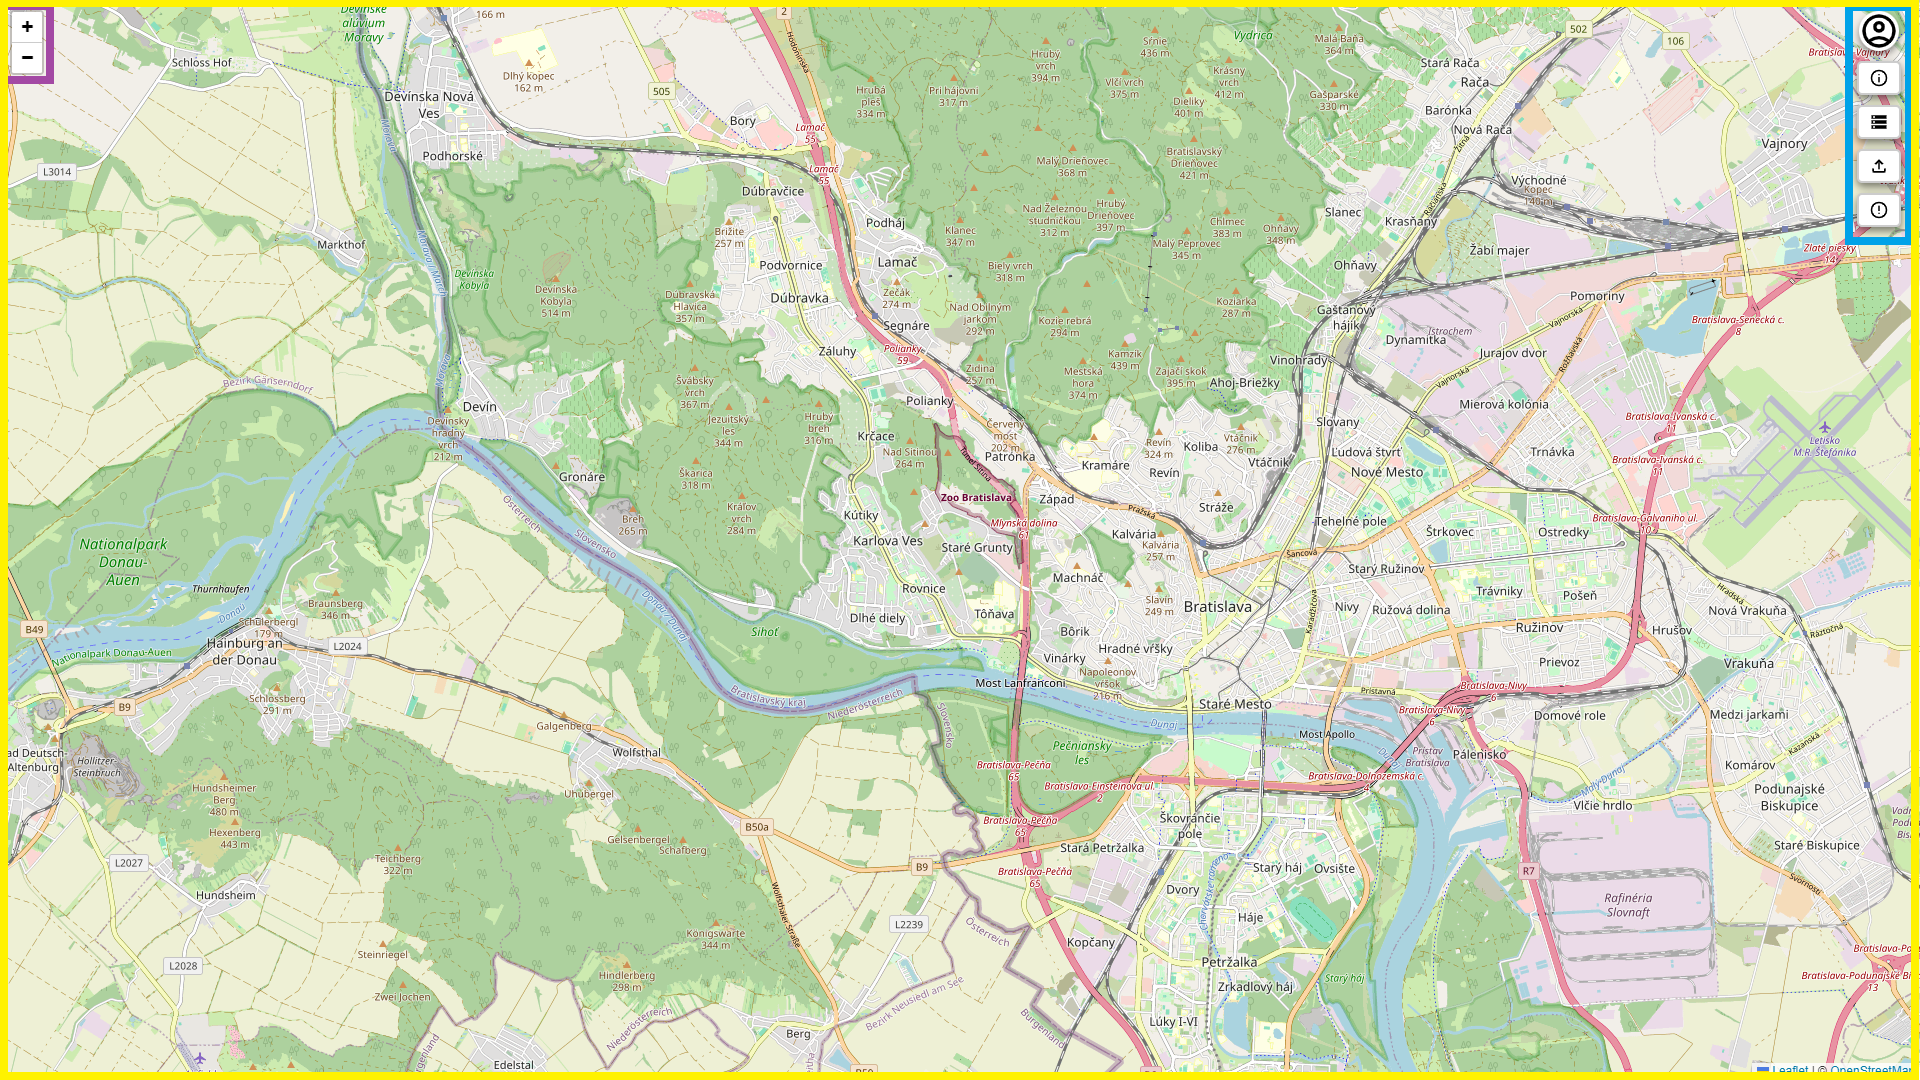
\includegraphics[width=0.9\textwidth]{img/map.png}
  \caption{Stránka s mapou}
  \label{fig:map}
\end{figure}

\noindent\textbf{Mapa}\\
\indent Pomocou \acrshort{html} je definovaný \textit{div} tag, ktorý je prázdny. Má nastavený identifikátor s hodnotou \textit{``map''}. Mapa je inicializovaná pomocou \textit{Leaflet} knižnice\cite{leaflet}. Pri inicializácii konštruktora mapy sa poskytuje identifikátor HTML elementu \textit{div} a nastavujú sa súradnice pre zobrazenie mapy. V súčasnosti je predvolená konfigurácia mapy nastavená tak, aby zobrazovala Bratislavu, pričom stred mapy sa nachádza v Mlynskej Doline v Bratislave. Po inicializácií bude mapa zobrazená na stránke. Je responzívna, takže pri rôznych veľkostiach displejov alebo pri rôznych veľkostiach okna je mapa vždy zobrazená na celej stránke.  Trasy na mape sú zobrazené modrou a červenou čiarou. Červenou čiarou sú zobrazené pôvodné trasy a modrou farbou trasy pripnuté k cestnej sieti. Pri prejdení myšou ponad zobrazené trasy sa zobrazí okno, ktoré obsahuje trasy ležiace pod ukazovateľom myši. Táto funkcionalita je implementovaná z dôvodu, že po pripnutí môže na jednej ceste ležať niekoľko trás.  \\

\noindent\textbf{Tlačidlá na priblíženie mapy}\\
\indent Tlačidlá na priblíženie sú súčasťou mapy a poloha tlačidiel je nastavená pomocou \textit{Leaflet} knižnice\cite{leaflet}. Tlačidlo s označením '\textit{+}' slúži na priblíženie mapy a '\textit{-}' slúži na oddialenie. Na počítačoch je možné mapu priblížiť alebo oddialiť pomocou rolovacieho kolieska na myši. Na mobilných zariadeniach sa tento efekt dosiahne gestom priblíženia alebo oddialenia, potiahnutím prstami po obrazovke. Mapu je možné priblížiť aj dvojklikom, či už na mobilnom zariadení alebo počítači.\\

\noindent\textbf{Panel akcii}\\
\indent Panel sa skladá z niekoľkých tlačidiel, ktoré vykonajú po kliknutí rôzne akcie:
\begin{itemize}
  \item Profile 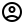
\includegraphics{img/icons/profile.png} \footnotemark{}
  \item About 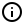
\includegraphics{img/icons/info.png} \footnotemark[\value{footnote}]
  \item Show Files 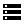
\includegraphics{img/icons/files.png} \footnotemark[\value{footnote}]
  \item Upload File 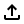
\includegraphics{img/icons/upload.png} \footnotemark[\value{footnote}]
  \item Error Files 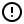
\includegraphics{img/icons/error.png} \footnotemark[\value{footnote}]
\end{itemize}

\footnotetext{Obrázok prevzaný z \textit{https://fonts.google.com/icons}.}

Po kliknutí na tlačidlo \textit{Profile} sa otvorí  okno, ktoré zobrazuje uvítaciu hlášku s používateľským menom. Taktiež obsahuje prepínač, ktorý nastavuje, či sa má mapa prispôsobiť zobrazeným trasám pri zobrazení alebo skrytí trasy a tlačidlo, ktoré po kliknutí odhlási používateľa. Okno je zobrazené na obrázku \ref{fig:profile_dialog}.

\begin{figure}[H]
  \centering
  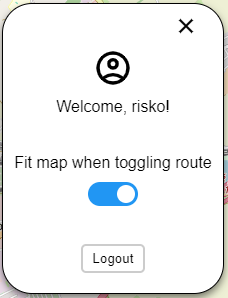
\includegraphics[width=0.2 \textwidth]{img/tools-panel/profile-dialog.png}
  \caption{Dialógové okno zobrazené po kliknutí \textit{Profile} tlačidla.}
  \label{fig:profile_dialog}
\end{figure}

Tlačidlo \textit{About} používateľa presmeruje na druhú stránku, kde je možné vidieť informácie o webovej aplikácii spolu s návodom na použitie aplikácie.

Pre zobrazenie nahraných súborov používateľ klikne na tlačidlo \textit{Show Files}. Otvorí sa dialógové okno viditeľné na obrázku \ref{fig:uploaded_routes_dialog}, ktoré zobrazí zoznam nahraných súborov v tabuľke. Riadok v tabuľke reprezentuje nahraný súbor.
\begin{figure}[H]
  \centering
  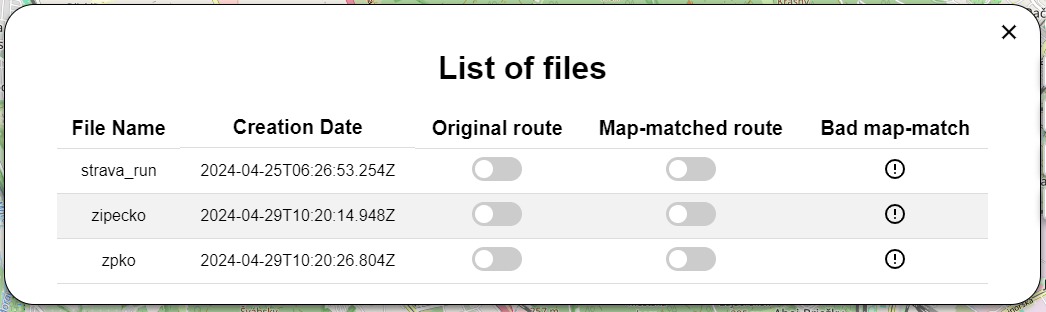
\includegraphics[width=0.8 \textwidth]{img/tools-panel/uploaded-routes.png}
  \caption{Dialógové okno zobrazené po kliknutí \textit{Show Files} tlačidla.}
  \label{fig:uploaded_routes_dialog}
\end{figure}
\noindent Tabuľka obsahuje stĺpce:
\begin{itemize}
  \item File Name - Názov nahraného ZIP súboru. Po kliknutí na názov súboru sa otvorí nové dialógové okno, ktoré zobrazuje trasy, ktoré nahraný ZIP súbor obsahuje
        \begin{figure}[H]
          \centering
          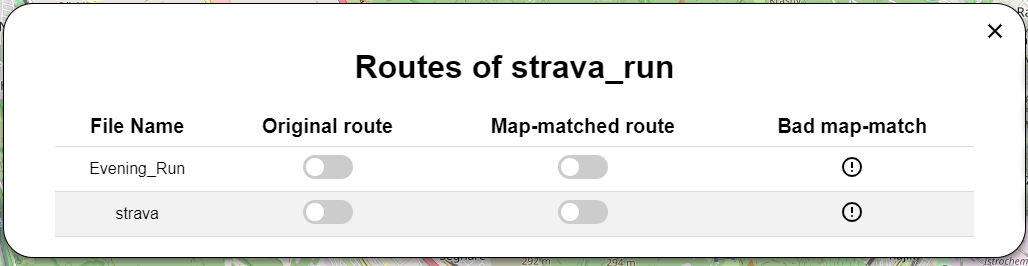
\includegraphics[width=0.8 \textwidth]{img/tools-panel/routes-of-zip.png}
          \caption{Dialógové okno zobrazené po kliknutí na názov nahraného ZIP súboru.}
        \end{figure}
  \item Creation Date - Dátum a čas, kedy bol ZIP súbor spracovaný
  \item Original route - Prepínač, ktorý zobrazí na mape všetky pôvodné trasy, ktoré ZIP súbor obsahuje
  \item Map-matched route - Prepínač, ktorý zobrazí na mape všetky trasy pripnuté k cestnej sieti, ktoré ZIP súbor obsahuje
  \item Bad map-match - Ak trasa nie je správne pripnutá k cestnej sieti, stlačením tlačidla používateľ odošle informácie správcovi systému. Informácie zahŕňajú názov trasy, názov nahraného súboru a používateľské meno
\end{itemize}

Po kliknutí na tlačidlo \textit{Upload file} sa otvorí dialógové okno, ktoré obsahuje vstupné polia a tlačidlo. V okne sú tri vstupné polia typu \textit{slider}, ktoré nastavujú parametre pripnutia trasy k cestnej sieti. Každý parameter je nastavený na predvolenú hodnotu, no používateľ môže hodnotu meniť. K jednotlivým parametrom sú vysvetlivky, ktoré sú zobrazené po prejdení myšou po ikone 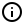
\includegraphics[scale=0.5]{img/icons/info.png}. Posledné vstupné pole slúži na výber ZIP súboru. Nahranie súboru je nutné potvrdiť stlačením tlačidla \textit{Upload}.
\begin{figure}[H]
  \centering
  
\includegraphics[width=1 \textwidth]{img/tools-panel/upload-dialog.png}
  \caption{Dialógové okno zobrazené po kliknutí \textit{Upload File} tlačidla.}
\end{figure}

Pre zobrazenie chybových nahraných súborov používateľ klikne na tlačidlo \textit{Error Files}. Kliknutím otvorí dialógové okno, ktoré pomocou tabuľky zobrazí nahrané ZIP súbory, v ktorých sa pri pripínaní trás k cestnej sieti vyskytla chyba. Každý riadok v tabuľke reprezentuje nahraný súbor. Tabuľka obsahuje stĺpce:
\begin{itemize}
  \item File Name - Názov nahraného ZIP súboru
  \item Download zip - Tlačidlo, ktorým je možné stiahnuť nahraný ZIP súbor. Je zobrazené vždy, keď je na serveri nahraný ZIP súbor. Nie je zobrazené iba v špeciálnom prípade, kedy sa používateľ pripojí na server pomocou \textit{\acrshort{ftp}} a nahrá súbory na server bez komprimovania trás do ZIP súboru.
  \item Rerun map-matching - Tlačidlo, ktorým sa znovu-spustí algoritmus pripínania trás k cestnej sieti. Je viditeľné vždy, keď je v priečinku používateľa rozbalený nahraný ZIP súbor. Nie je zobrazené len v prípade, že sa nahraný súbor nepodarilo rozbaliť.
  \item Delete zip and unzipped files - Tlačidlá, ktoré vymažú zo servera nahraný ZIP súbor, alebo rozbalený ZIP súbor. Sú zobrazené pod podmienkou, že sa na serveri nachádza v priečinku používateľa rozbalený ZIP súbor, alebo/aj samotný ZIP súbor.
\end{itemize}
Ukážku okna je možné vidieť na obrázku nižšie.
\begin{figure}[H]
  \centering
  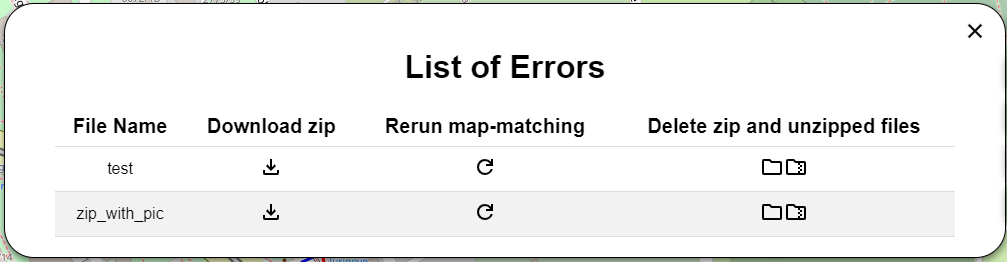
\includegraphics[width=1 \textwidth]{img/tools-panel/errors-dialog.png}
  \caption{Dialógové okno zobrazené po kliknutí \textit{Error Files} tlačidla.}
\end{figure}
\noindent Po znovu-spustení algoritmu pripínania trás k cestnej sieti je po úspešnom pripnutí nutné manuálne vymazať nahraný ZIP súbor a rozbalené súbory ZIP súboru tlačidlami zobrazenými v \textit{Delete zip and unzipped files}.
